\documentclass[]{article}

\usepackage[margin=2cm]{geometry}
\usepackage{graphicx} % Allows including images
\usepackage{booktabs} % Allows the use of \toprule, \midrule and \bottomrule in tables
\usepackage{textcomp}
\usepackage{threeparttable}
\usepackage{tikz}
\usepackage[utf8]{inputenc}
\usepackage{makecell}
\usepackage{marvosym}
\usepackage{eurosym}
\usepackage{threeparttablex}
\usepackage{tabularx}
\usepackage{subcaption} % For subfigures with captions
\usepackage{float} % Provides the [H] placement option
\DeclareUnicodeCharacter{20AC}{\EUR{}}
\usepackage[normalem]{ulem}

%opening
\title{Family Risk Sharing}
\author{B-C-V}

\begin{document}

\maketitle

\section{Summary statistics and life-cycle behavior}

%Summary statistics
\begin{table}[h]\centering
	
	\caption{Summary statistics}
	\label{table:sum_stat}
	\begin{threeparttable}[t]\centering
		\begin{tabular*}{\textwidth}{l@{\extracolsep{\textwidth minus \textwidth}}ccccc}
			\toprule
			& Household& Household  & Wife, Private & Husband, Private & Home good  \\
        	& assets  & earnings  & consumption & consumption & expenditure  \\[0.5ex]			&  (1)& (2) & (3) & (4) & (5)   \\[0.5ex]
			\midrule		
			Mean          & 4.115 & 1.742 & 0.152 & 0.265 & 1.501    \\ Gini          & 0.664 & 0.450 & 0.410 & 0.286 & 0.230    \\ Top 1\% share & 0.066 & 0.044 & 0.043 & 0.029 & 0.023    \\\bottomrule    
			\\[-2.5ex] 
		\end{tabular*}
		\begin{tablenotes}[flushleft]
			\footnotesize{\item \textsc{Notes}: assets and earnings are measure across the population regardless of marital status, while other variables are measured among married households.
			}
		\end{tablenotes}
	\end{threeparttable}
\end{table}


%Life-cycle behavior
\begin{figure}[H]
	\centering
	% First picture
	\begin{subfigure}{0.49\textwidth} % Adjust width as needed
		\centering
		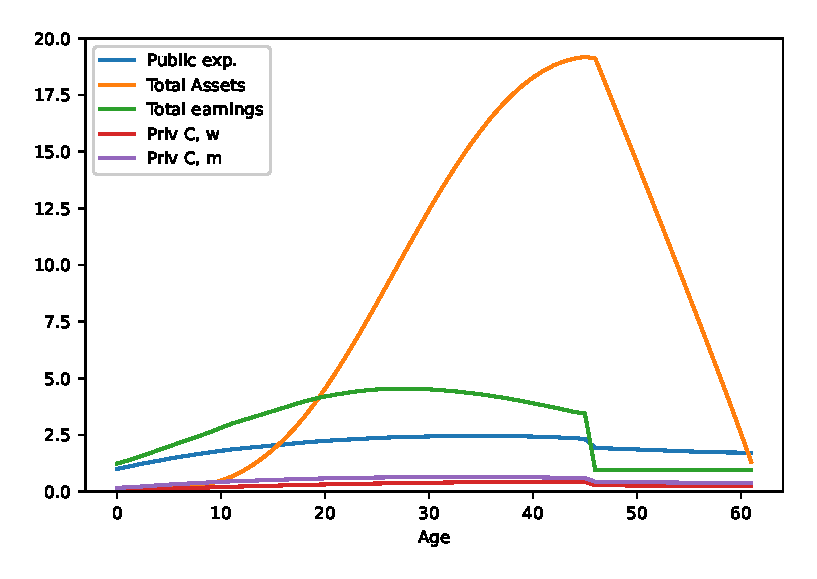
\includegraphics[width=\textwidth]{lifecycle_aggregate.eps} % Replace with your first pgf file name
		\caption{Married couples + single women}
		\label{fig:picture1}
	\end{subfigure}
	% Second picture
	\begin{subfigure}{0.49\textwidth}
		\centering
		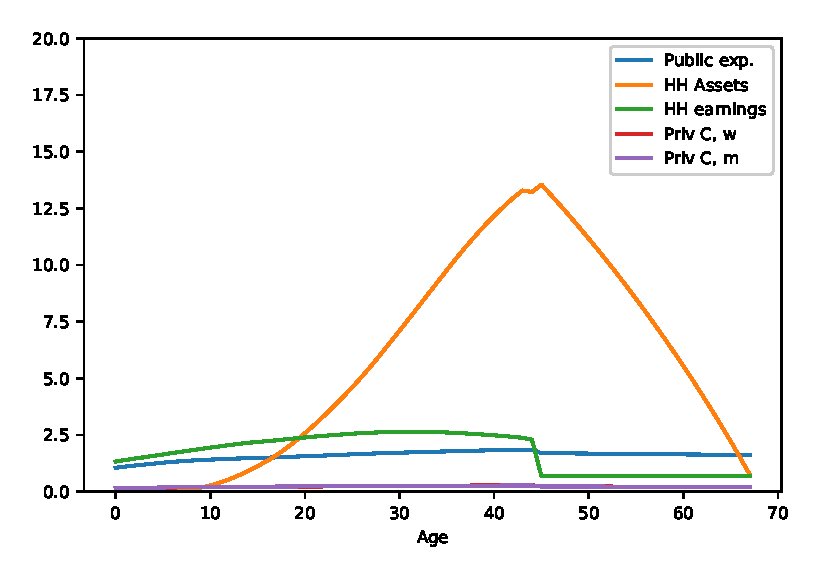
\includegraphics[width=\textwidth]{lifecycle_married.eps} % Replace with your second pgf file name
		\caption{Married couples}
		\label{fig:picture2}
	\end{subfigure}
	% Third picture
	\begin{subfigure}{0.49\textwidth}
		\centering
		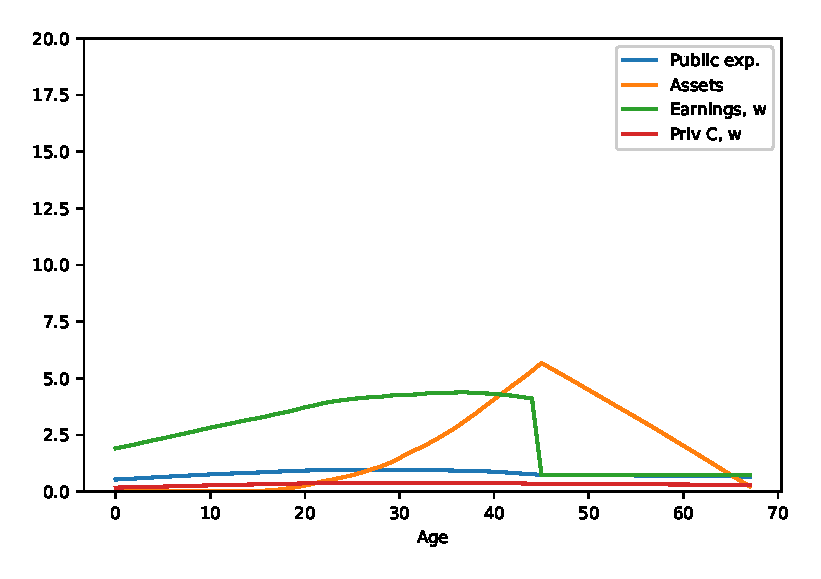
\includegraphics[width=\textwidth]{lifecycle_singlew.eps} % Replace with your third pgf file name
		\caption{Single women}
		\label{fig:picture3}
	\end{subfigure}
	
	\caption{Life-cycle behavior of different types of household, averages}
	\label{fig:all_pictures}
\end{figure}

\section{Marital surplus, renegotiation and divorce}

% distribution of marital surplus



%Marital surplus, renegotiations and divorce

\begin{figure}[H]
	\centering
	% First picture
	\begin{subfigure}{0.49\textwidth} % Adjust width as needed
		\centering
		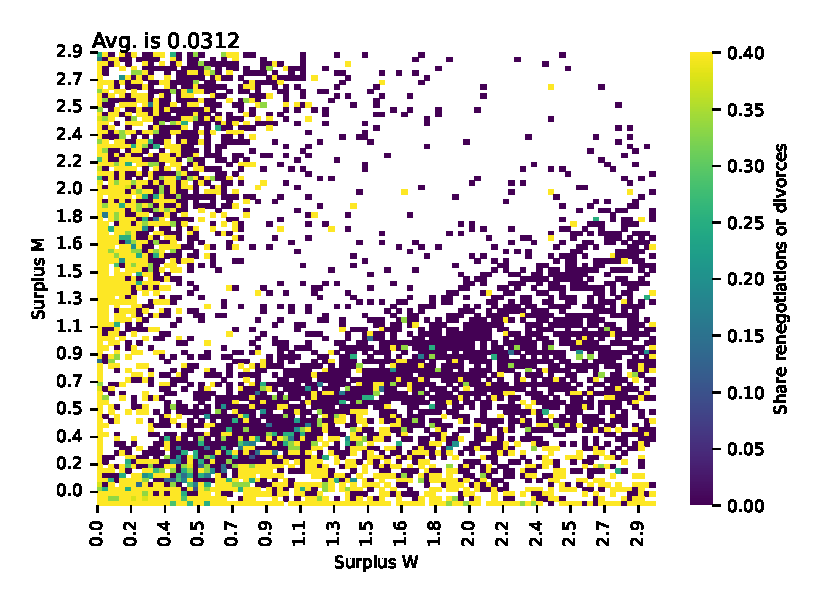
\includegraphics[width=\textwidth]{surp_ren_div.eps} % Replace with your first pgf file name
		\caption{Renegotiations and divorces}
		\label{fig:picture1}
	\end{subfigure}
	% Second picture
	\begin{subfigure}{0.49\textwidth}
		\centering
		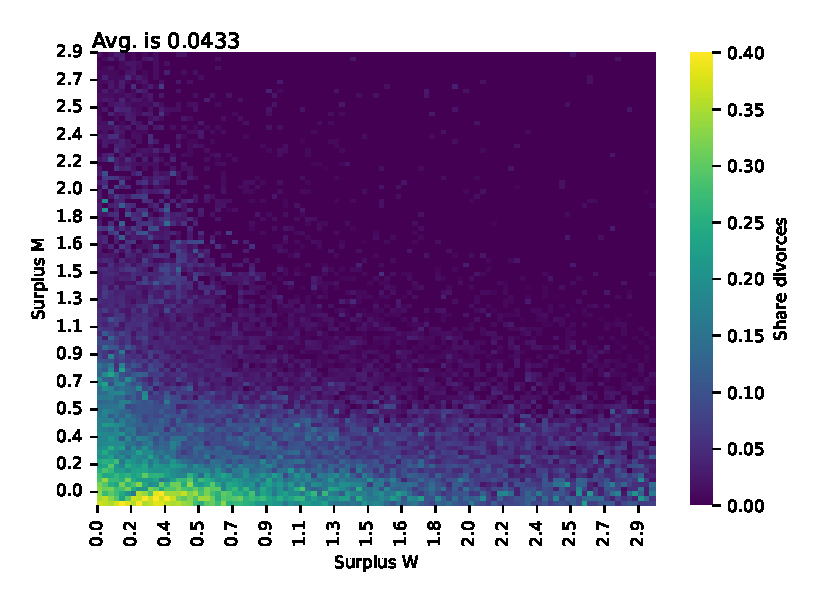
\includegraphics[width=\textwidth]{surp_div.eps} % Replace with your second pgf file name
		\caption{Divorces}
		\label{fig:picture2}
	\end{subfigure}
	% Third picture
	\begin{subfigure}{0.49\textwidth}
		\centering
		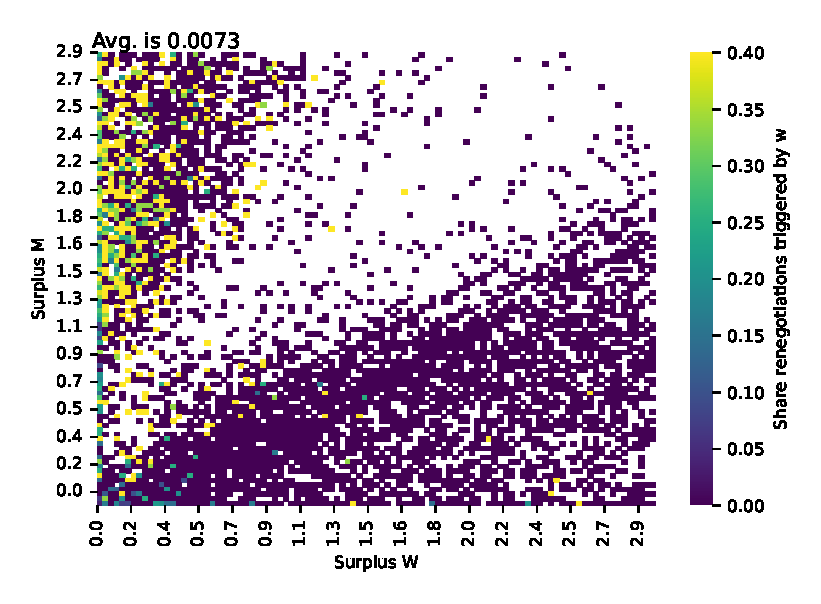
\includegraphics[width=\textwidth]{surp_renw.eps} % Replace with your third pgf file name
		\caption{Renegotiations triggered by the wife}
		\label{fig:picture3}
	\end{subfigure}
		% Third picture
	\begin{subfigure}{0.49\textwidth}
		\centering
		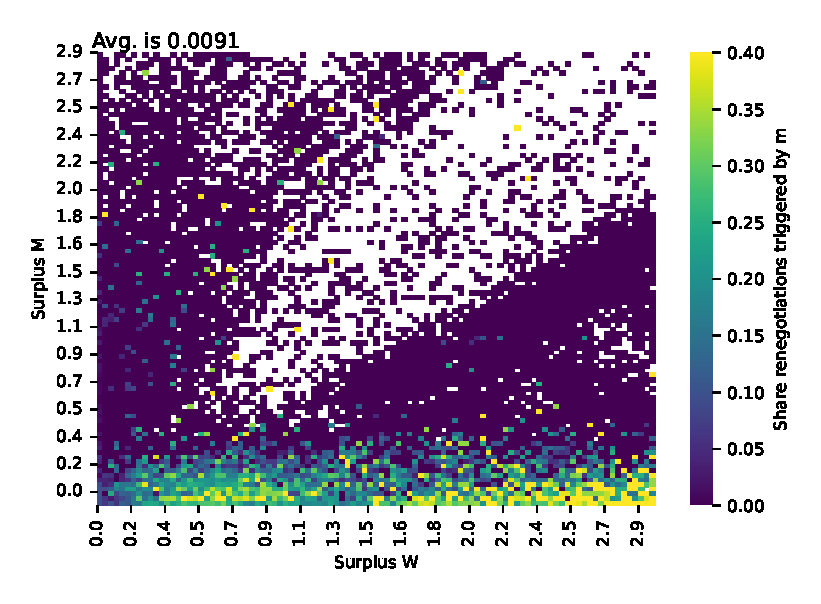
\includegraphics[width=\textwidth]{surp_renm.eps} % Replace with your third pgf file name
		\caption{Renegotiation triggered by the husband}
		\label{fig:picture3}
	\end{subfigure}
	
	\caption{Marital surplus, renegotiation and divorce}
	\label{fig:surp_ren}
\end{figure}

\begin{figure}[H]
	\centering
	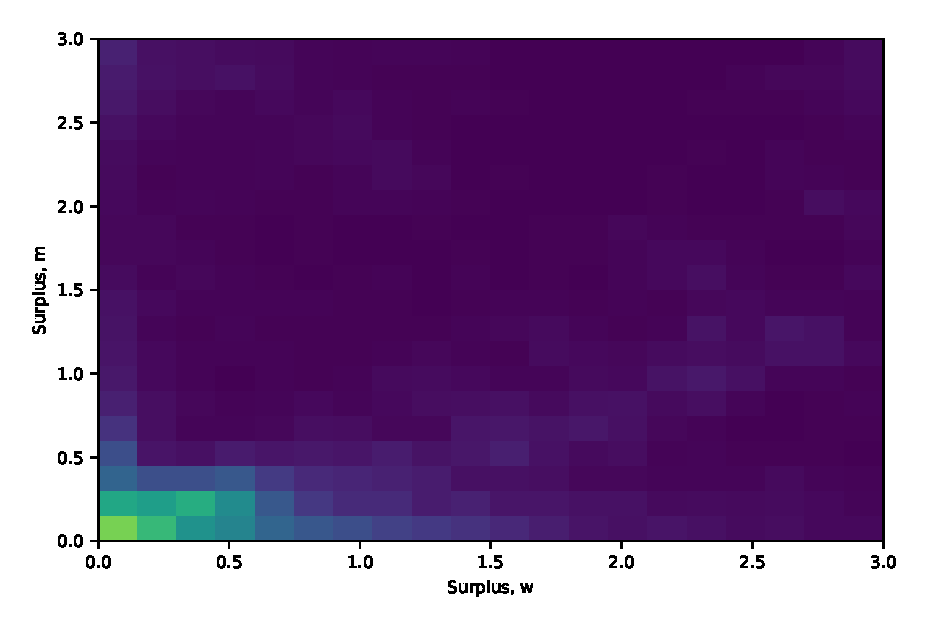
\includegraphics[width=\textwidth]{surplus_dist.eps} 
	\caption{Marital surplus distribution (value of staying married - value of divorce)}
	\label{fig:surplus dist}
\end{figure}

% distribution of marital surplus
\begin{figure}[H]
	\centering
	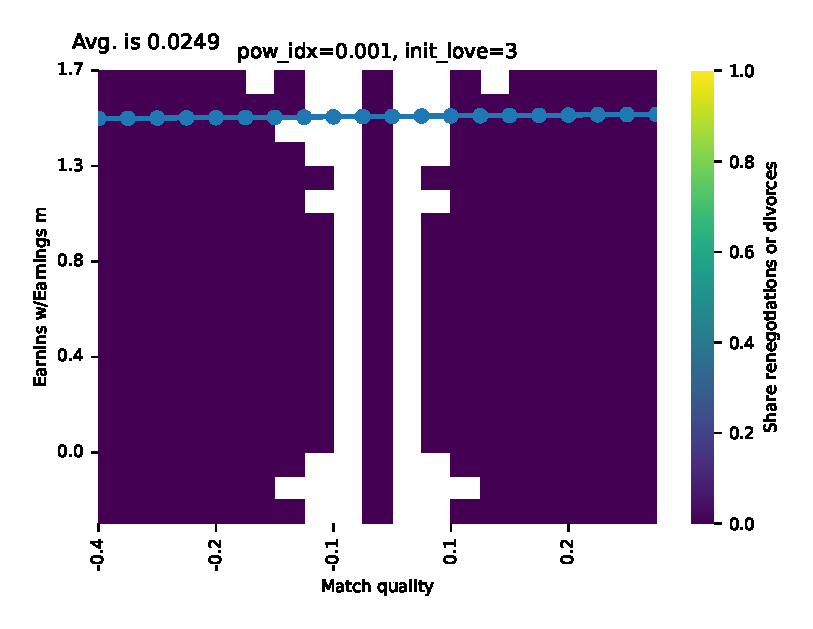
\includegraphics[width=\textwidth]{match_earn_ren_div.eps} 
	\caption{Share or divorces and renegotiations given relative earnings and match quality}
	\label{fig:surplus match earn}
\end{figure}


\section{Consumption insurance regressions}
%%%%%%%%%%%%%%%%%%%%%%%%
%All income
%%%%%%%%%%%%%%%%%%%%%%%
\begin{table}[h]\centering
	
	\caption{Pass-through of changes in income on consumption and consumption shares, using changes in...}
	\label{table:allinc}
	\begin{threeparttable}[t]\centering
		\begin{tabular*}{\textwidth}{l@{\extracolsep{\textwidth minus \textwidth}}ccccc}
			\toprule
			& Total Exp  & Common Exp  & Husband Exp & Wife Exp & Wife share  \\[0.5ex]
			&  (1)& (2) & (3) & (4) & (5)   \\[0.5ex]
			\midrule		
			...total income   & \textbf{0.404} & 0.367 & & &    \\ ...wife income    & 0.170 & 0.165&  \textbf{0.143} &  \textbf{0.227} &  \textbf{0.084}    \\ ...husband income & 0.194 &  0.191&  \textbf{0.215} &  \textbf{0.184} &  \textbf{-0.031}    \\\bottomrule    
			\\[-2.5ex] 
		\end{tabular*}
		\begin{tablenotes}[flushleft]
			\footnotesize{\item \textsc{Notes}: Coefficient interpretation: 1\% change in income leads to X\% change in expenditure. Coefficients associated to changes in the wife income are computed using women working in two consecutive periods.
			}
		\end{tablenotes}
	\end{threeparttable}
\end{table}



%%%%%%%%%%%%%%%%%%%%%%%%
%Transitory income changes
%%%%%%%%%%%%%%%%%%%%%%%
\begin{table}[h]\centering
	
	\caption{Pass-through of changes in income on consumption and consumption shares, using \textbf{transitory
		} changes in...}
	\label{table:trainc}
	\begin{threeparttable}[t]\centering
		\begin{tabular*}{\textwidth}{l@{\extracolsep{\textwidth minus \textwidth}}ccccc}
			\toprule
			& Total Exp  & Common Exp  & Husband Exp & Wife Exp & Wife share  \\[0.5ex]
			&  (1)& (2) & (3) & (4) & (5)   \\[0.5ex]
			\midrule		
			...total income   & \textbf{0.054} & 0.051 & & &    \\ ...wife income    & 0.040 & 0.039&  \textbf{0.045} &  \textbf{0.044} &  \textbf{0.000}    \\ ...husband income & 0.054 &  0.052&  \textbf{0.072} &  \textbf{0.013} &  \textbf{-0.048}    \\\bottomrule    
			\\[-2.5ex] 
		\end{tabular*}
		\begin{tablenotes}[flushleft]
			\footnotesize{\item \textsc{Notes}: Coefficient interpretation: 1\% change in income leads to X\% change in expenditure. Coefficients associated to changes in the wife income are computed using women working in two consecutive periods.
			}
		\end{tablenotes}
	\end{threeparttable}
\end{table}

%%%%%%%%%%%%%%%%%%%%%%%%%%%
%Persistent income changes
%%%%%%%%%%%%%%%%%%%%%%%%%%
\begin{table}[h]\centering
	
	\caption{Pass-through of changes in income on consumption and consumption shares, using \textbf{persistent} changes in...}
	\label{table:persinc}
	\begin{threeparttable}[t]\centering
		\begin{tabular*}{\textwidth}{l@{\extracolsep{\textwidth minus \textwidth}}ccccc}
			\toprule
			& Total Exp  & Common Exp  & Husband Exp & Wife Exp & Wife share  \\[0.5ex]
			&  (1)& (2) & (3) & (4) & (5)   \\[0.5ex]
			\midrule		
			...total income   & \textbf{0.321} & 0.308 & & &    \\ ...wife income    & 0.346 & 0.339&  \textbf{0.313} &  \textbf{0.504} &  \textbf{0.191}    \\ ...husband income & 0.330 &  0.322&  \textbf{0.390} &  \textbf{0.322} &  \textbf{-0.068}    \\\bottomrule    
			\\[-2.5ex] 
		\end{tabular*}
		\begin{tablenotes}[flushleft]
			\footnotesize{\item \textsc{Notes}: Coefficient interpretation: 1\% change in income leads to X\% change in expenditure. Coefficients associated to changes in the wife income are computed using women working in two consecutive periods.
			}
		\end{tablenotes}
	\end{threeparttable}
\end{table}

%%%%%%%%%%%%%%%%%%%%%%%%
%BPP MPC
%%%%%%%%%%%%%%%%%%%%%%%
\begin{table}[h]\centering
	
	\caption{MPC calculated as in BPP, using transitory changes in...}
	\label{table:BPP_MPC}
	\begin{threeparttable}[t]\centering
		\begin{tabular*}{\textwidth}{l@{\extracolsep{\textwidth minus \textwidth}}cccc}
			\toprule
			& Total Exp  & Common Exp  & Husband Exp & Wife Exp  \\[0.5ex]
			&  (1)& (2) & (3) & (4)   \\[0.5ex]
			\midrule		
			...husband income & 0.031 & 0.030 & 0.037 & -0.011  \\ ...wife income    & 0.018 & 0.019 & 0.007 & 0.062  \\ ...total income   & 0.268 & 0.234 & 0.404 & 0.416  \\\bottomrule    
			\\[-2.5ex] 
		\end{tabular*}
		\begin{tablenotes}[flushleft]
			\footnotesize{\item \textsc{Notes}: the consumption insurance parameters displayed in the table are computed as $$\frac{E\left(\Delta c_t \Delta y_{t+1}\right)}{E\left(\Delta y_t \Delta y_{t+1}\right)},$$ where $y_t$ can the income of the husband, wife or the sum of the two (total). Variables $c_t$ can be the total, common, husband or wife' expenditures. Coefficients associated to changes in the wife income are computed using women working in two consecutive periods.
			}
		\end{tablenotes}
	\end{threeparttable}
\end{table}


%%%%%%%%%%%%%%%%%%%%%%%%
%BPP PERSISTENT
%%%%%%%%%%%%%%%%%%%%%%%
\begin{table}[h]\centering
	
	\caption{Consumption insurance to persistent income shocks, calculated as in BPP, using persistent changes in...}
	\label{table:BPP_PER}
	\begin{threeparttable}[t]\centering
		\begin{tabular*}{\textwidth}{l@{\extracolsep{\textwidth minus \textwidth}}cccc}
			\toprule
			& Total Exp  & Common Exp  & Husband Exp & Wife Exp  \\[0.5ex]
			&  (1)& (2) & (3) & (4)   \\[0.5ex]
			\midrule		
			...husband income & 0.370 & 0.365 & 0.418 & 0.354  \\ ...wife income    & 0.431 & 0.420 & 0.379 & 0.598  \\ ...total income   & 0.541 & 0.516 & 0.636 & 0.690  \\\bottomrule     
			\\[-2.5ex] 
		\end{tabular*}
		\begin{tablenotes}[flushleft]
			\footnotesize{\item \textsc{Notes}: the consumption insurance parameters displayed in the table are computed as $$\frac{E\left(\Delta c_t\left(\Delta y_{t-1}+\Delta y_t+\Delta y_t\right)\right)}{E\left(\Delta y_t\left(\Delta y_{t-1}+\Delta y_t+\Delta y_t\right)\right)},$$ where $y_t$ can the income of the husband, wife or the sum of the two (total). Variables $c_t$ can be the total, common, husband or wife' expenditures. Coefficients associated to changes in the wife income are computed using women working in two consecutive periods.
}
		\end{tablenotes}
	\end{threeparttable}
\end{table}

%%%%%%%%%%%%%%%%%%%%%%%%%%%%%%%%%%
%Income shocks and labor supply
%%%%%%%%%%%%%%%%%%%%%%%%%%%%%%%%%
\begin{table}[h]\centering
	
	\caption{Women's employment response (in percentage points) to different types of income shocks}
	\label{table:shocks_WLP}
	\begin{threeparttable}[t]\centering
		\begin{tabular*}{\textwidth}{@{\extracolsep{\textwidth minus \textwidth}}cccccc}
			\toprule
			  \multicolumn{2}{c}{Transitory shocks}  &  \multicolumn{2}{c}{Persistent shocks} & \multicolumn{2}{c}{Transitory+persistent shocks}   \\[0.5ex]
			
		    \cmidrule(lr){1-2}    \cmidrule(lr){3-4}  \cmidrule(lr){5-6} 
			
			
			
			 Wife  & Husband  &Wife  & Husband  & Wife  & Husband     \\[0.5ex]
			  (1)& (2) & (3) & (4) & (5)  & (6)  \\[0.5ex]
			\midrule		
			  0.000 & 0.000 & 0.000 & 0.000 & 0.000 & 0.000  \\\bottomrule     
			\\[-2.5ex] 
		\end{tabular*}
		\begin{tablenotes}[flushleft]
			\footnotesize{\item \textsc{Notes}: the income shocks relate to \textit{potential log income} $y$. In the case of women, a positive potential income shocks does not translate in more earnings if the women does not work. The numbers displayed in the table are OLS coefficients:
				
				$$\frac{E(\Delta y_t \  \Delta WLP_t)}{E(\Delta y_t)},$$
			
			where $\Delta WLP$ is the change in women's employment over two consecutive periods.
				
			}
		\end{tablenotes}
	\end{threeparttable}
\end{table}

%%%%%%%%%%%%%%%%%%%%%%%%
%Level
%%%%%%%%%%%%%%%%%%%%%%%
\begin{table}[h]\centering
	
	\caption{Pass-through of changes in income on consumption and consumption shares, using changes in...}
	\label{table:level}
	\begin{threeparttable}[t]\centering
		\begin{tabular*}{\textwidth}{l@{\extracolsep{\textwidth minus \textwidth}}ccccc}
			\toprule
			& Total Exp  & Common Exp  & Husband Exp & Wife Exp & Wife share  \\[0.5ex]
			&  (1)& (2) & (3) & (4) & (5)   \\[0.5ex]
			\midrule		
			...total income   & \textbf{0.193} & 0.189 & & &    \\ ...wife income    & 0.291 & 0.300&  \textbf{-0.007} &  \textbf{-0.002} &  \textbf{0.021}    \\ ...husband income & 0.128 &  0.115&  \textbf{0.010} &  \textbf{0.003} &  \textbf{-0.005}    \\\bottomrule    
			\\[-2.5ex] 
		\end{tabular*}
		\begin{tablenotes}[flushleft]
			\footnotesize{\item \textsc{Notes}: Coefficient interpretation: 1 yen change in income leads to X yen change in expenditure. 
			}
		\end{tablenotes}
	\end{threeparttable}
\end{table}
\end{document}
